\chapter{Konzeption}
\label{chapter:Konzeption}
In diesem Kapitel wird auf die fachliche Konzeption der Anwendung, die Konzeption des \ac{knn} sowie auf die Beschreibung und Wahl des geeignetsten Frameworks zur Programmierung des \ac{knn} eingegangen.

\section{Fachliche Konzeption der Anwendung} %Benedikt
\label{section:Fachliche Konzeption der Anwendung} %Benedikt

\subsection{Grundidee} %Benedikt
\label{subsection:Grundidee} %Benedikt

\subsection{Mockup} %Benedikt
\label{subsection:Mockup} %Benedikt

\begin{figure}[htbp]
\centering
		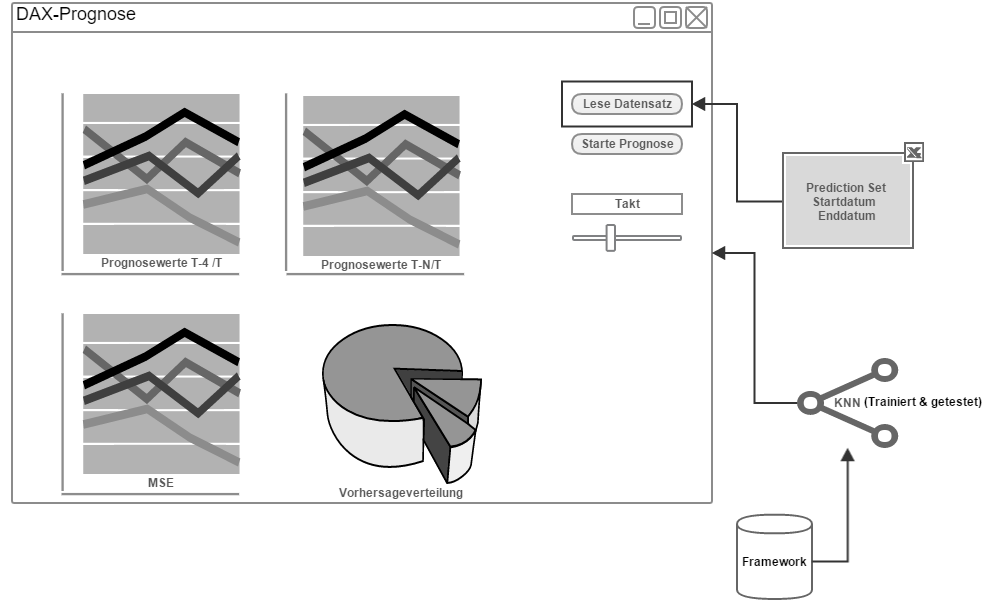
\includegraphics[width=0.95\textwidth]{mockup.PNG}
	\caption{Mockup der Anwendung}
	\label{fig:Mockup der Anwendung}
\end{figure}

\section{Konzeption des künstlichen neuronalen Netzes}
\label{section:Konzeption des künstlichen neuronalen Netzes}

In den folgenden drei Abschnitten wird auf die Konzeption des \ac{knn} eingegangen. Zunächst wird der Typ des \ac{knn} festgelegt. Anschließend wird die zugrundeliegende Topologie des \ac{knn} und das anzuwendende Lernverfahren bestimmt.

\subsection{Wahl des Netztyps}
\label{subsection:Wahl des Netztyps}

Grundsätzlich lassen sich \ac{knn} in zwei Oberklassen unterteilen. Die Hetero-Assoziativen Netze sowie die Auto-Assoziativen Netze. Hetero-Assoziative Netze bilden einen Vektor $A$ der Länge $n$ auf einem Vektor $B$ einer meist kürzeren Länge m $\{m \in \mathbb{N} | m \le n\}$ ab. Auto-Assoziative Netze wiederum bilden einen Eingabevektor der Länge $n$ auf einem Ausgabevektor der gleichen Länge ab. Innerhalb dieser zwei Klassen lassen sich \ac{knn} wiederum in mehrere Modelle aufteilen.Die folgende Tabelle liefert eine Übersicht der bekanntesten Modelle von \ac{knn} unterteilt in Klassen:

\begin{center}
\begin{tabular}{|c|c|}
\hline 
 Hetero- assoziative Netzmodelle & Auto-assoziative Netzmodelle \\ 
\hline 
(M)Adaline & Hopfield-Netze \\ 
\hline  
Perzeptron &  Boltzmann Maschinen \\ 
\hline 
Multilayerperzeptron & - \\ 
\hline 
\end{tabular} 
\end{center}

Da es sich bei dem \ac{dax}-Kurs um einen skalaren Wert handelt, der aufgrund mehrerer vorhergehender \ac{dax}-Kurse prognostiziert wird, wir ein Netzmodell aus der Klasse der Hetero-Assoziativen Netze benötigt. Für die Anwendung ist demnach nur die linke Spalte der Tabelle relevant. 

Für den nächsten Auswahlschritt können die folgenden zwei Theoreme betrachtet werden:

\newtheorem*{theorem2*}{Theorem der linearen Separierbarkeit}
\begin{theorem2*}
Seien $X_{0}$ and $X_{1}$ zwei Datenmengen im $n$-dimensionalen euklidischen Raum. Dann sind die Mengen $X_{0}$ and $X_{1}$ genau dann als "`linear separierbar"', wenn es  $n+1$ Werte $w_{1}, w_{2},..,w_{n}, k$, gibt, sodass jeder Punkt  $x \in X_{0}$ die Bedingung $\sum^{n}_{i=1} w_{i}x_{i} > k$ erfüllt und jeder Punkt $x \in X_{1}$ die Bedingung $\sum^{n}_{i=1} w_{i}x_{i} < k$ erfüllt.
\end{theorem2*}

Da es sich beim Börsenkurs auf Grund des obigen Theorems um eine nicht linear separierbare Funktion handelt, das Perzeptron und die Adaline aber nur linear separierbare Funktionen approximieren können, fallen diese Möglichkeiten weg. Nicht jedoch das mehrschichtige vorwärtsgerichtete Netz. Das dieses \ac{knn} auch tatsächlich dafür geeignet ist, belegt das folgende Theorem:


\newtheorem*{theorem1*}{Theorem von Kolmogorov}
\begin{theorem1*}
Für ${n \in \mathbb{N} | n>2}$ lässt sich jede reellwertige Funktion $f:[0;1]^n\rightarrow[0;1]$ durch ein dreischichtiges vorwärtsverknüpftes Netz mit maximal $n$ Einheiten in der Eingabeschicht,$(2n+1)$ Einheiten in der Zwischenschicht und $2n+1$ Einheiten in der Ausgabeschicht berechnen.
\end{theorem1*}

Ein Börsenkurs kann prinzipiell jede beliebige Funktion annehmen. Durch das obige Theorem ist jedoch sichergestellt, dass das mehrschichtige vorwärstgerichtete Netz in der Lage ist, diese Funktionen zu approximieren.


\subsection{Wahl der Grundlegenden Topologie}
\label{subsection:Wahl Grundlegenden Topologie}

Zur Prognose werden die vier vergangegen Daten zur Prognose des zukünftigen Wertes als Input Layer genutzt. Da das Ergebnis ein skalarer Wert ist, wir nur ein neurona als Output Layer benötigt. Die optimale Größe des Hidden Layers wird in Punkt (Kapitelverweis) ermittelt. Somit sieht die Topoligie des knn bis jetzt wie golfr aus:

\begin{figure}[H]
\centering
		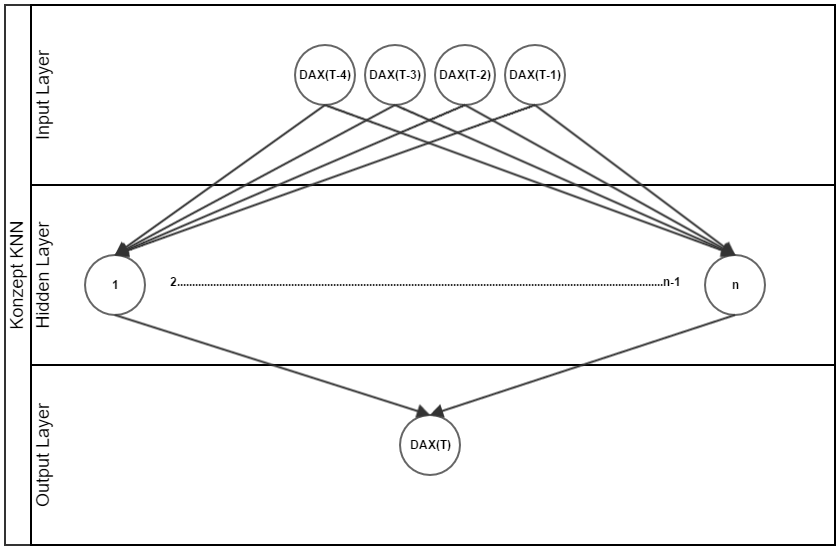
\includegraphics[width=0.95\textwidth]{KonzeptKNN.PNG}
	\caption{Grundlegendes Konzept des KNN}
	\label{fig:Grundlegendes Konzept des KNN}
\end{figure}

\subsection{Wahl des Lernverfahrens} 
\label{subsection:Wahl des Lernverfahrens} 


\section{Beschreibung von KNN-Frameworks} %Benedikt
\label{section:Beschreibung von Frameworks} %Benedikt

\subsection{SNNS} %Benedikt
\label{subsection:SNNS} %Benedikt

\subsection{JavaNNS}  %Benedikt
\label{subsection:JavaNNS}  %Benedikt

\subsection{Neuroph} %Benedikt
\label{subsection:Neuroph} %Benedikt

\section{Wahl des geeignetsten Frameworks} %Benedikt
\label{section:Wahl des geeignetsten Frameworks} %Benedikt

